% Original exercises -- sessions 47 to 55 (chapter 7: discrete random
% variables and the binomial distribution; chapter 8: revision and consolidation).
% Format: \DefExo{session}{target}{statement}{detailed solution}{answer lines}

% -----------------------------------------------------------------------------
% Chapter 7 -- Discrete random variables and the binomial distribution
% -----------------------------------------------------------------------------
\DefExo{47}{Distribution of a gain and expected value}{%
To launch a new perfume, a cosmetics chain sells its customers a scratch card for €$3$. The cards are printed in booklets of $25$: in each booklet, $16$ cards are losing cards, $6$ cards give a €$6$ shopping voucher and $3$ cards give a €$13$ shopping voucher. A customer buys a card chosen at random from a new booklet.

Let $G$ be the random variable equal to the customer's net gain, in euros, that is, the value of the voucher obtained minus the price of the card (a negative gain is a loss).
\begin{enumerate}
\item What values does $G$ take?
\item Copy and complete the following table, which gives the probability distribution of $G$.
\begin{center}
\renewcommand{\arraystretch}{1.4}
\begin{tabular}{|l|*{3}{p{1.7cm}|}}
\hline
Value $g_i$ of $G$ & & & \\
\hline
$P(G=g_i)$ & & & \\
\hline
\end{tabular}
\end{center}
\item Calculate the expected value $E(G)$. What can be said from the customer's point of view? And from the chain's point of view?
\item The chain wants to earn €$0.40$ on average per card sold, without changing the composition of the booklets. At what price should it sell the card?
\end{enumerate}
}{%
\begin{enumerate}
\item A losing card gives $G=0-3=-3$; a €$6$ voucher gives $G=6-3=3$; a €$13$ voucher gives $G=13-3=10$. So $G$ takes the values $-3$, $3$ and $10$.
\item The card is chosen at random among $25$ cards: all outcomes are equally likely.
\[
\begin{array}{|l|c|c|c|}\hline
g_i&-3&3&10\\\hline
P(G=g_i)&\dfrac{16}{25}=0.64&\dfrac{6}{25}=0.24&\dfrac{3}{25}=0.12\\\hline
\end{array}
\]
Check: $0.64+0.24+0.12=1$.
\item $E(G)=-3\times0.64+3\times0.24+10\times0.12=-1.92+0.72+1.20=0$.
The expected value is zero: over a large number of cards, the customer neither wins nor loses on average; the game is fair. The chain earns nothing on average from the cards themselves: the operation only serves to attract customers.
\item Let $B$ be the value of the voucher. $E(B)=0\times0.64+6\times0.24+13\times0.12=1.44+1.56=3$ euros. If the card costs $c$ euros, the customer's net gain is $B-c$ and its expected value is $3-c$ (each value of $G$ is decreased by $c$). We want $3-c=-0.40$, so $c=3.40$ euros.
Check: the values become $-3.40$, $2.60$, $9.60$ and $-3.40\times0.64+2.60\times0.24+9.60\times0.12=-2.176+0.624+1.152=-0.40$.
\end{enumerate}
}{5}

\DefExo{48}{Recognising a binomial distribution, n = 2}{%
On a large online sales platform, $12\,\%$ of shipped parcels are returned by the customer. The quality department chooses two shipped parcels at random. The number of shipped parcels is large enough for this choice to be treated as two random draws with replacement.

Let $R$ be the event ``the parcel is returned'' and $X$ the random variable equal to the number of returned parcels among the two chosen parcels.
\begin{center}
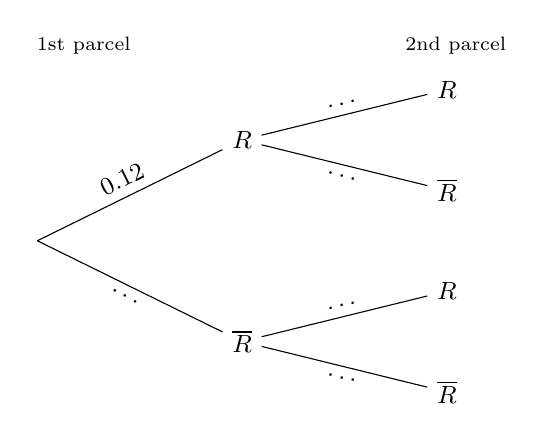
\begin{tikzpicture}[font=\small,x=26mm,y=8mm]
\coordinate (O) at (0,0);
\node (R1) at (1,1.6) {$R$};
\node (N1) at (1,-1.6) {$\overline R$};
\node (RR) at (2,2.4) {$R$};
\node (RN) at (2,0.8) {$\overline R$};
\node (NR) at (2,-0.8) {$R$};
\node (NN) at (2,-2.4) {$\overline R$};
\draw (O)--node[above,sloped]{$0.12$}(R1);
\draw (O)--node[below,sloped]{$\dots$}(N1);
\draw (R1)--node[above,sloped]{$\dots$}(RR);
\draw (R1)--node[below,sloped]{$\dots$}(RN);
\draw (N1)--node[above,sloped]{$\dots$}(NR);
\draw (N1)--node[below,sloped]{$\dots$}(NN);
\node[anchor=west,font=\scriptsize] at (-0.05,3.1) {1st parcel};
\node[anchor=west,font=\scriptsize] at (1.75,3.1) {2nd parcel};
\end{tikzpicture}
\end{center}
\begin{enumerate}
\item Copy and complete the weighted tree above.
\item Justify that $X$ follows a binomial distribution and give its parameters.
\item Calculate $P(X=0)$, $P(X=1)$ and $P(X=2)$. For $P(X=1)$, state how many paths of the tree give the event $\{X=1\}$.
\item Deduce, in two different ways, the probability that at least one of the two parcels is returned.
\end{enumerate}
}{%
\begin{enumerate}
\item First level: $P(R)=0.12$ and $P(\overline R)=1-0.12=0.88$. Since the draws are treated as draws with replacement, the second level uses the same probabilities: $0.12$ towards $R$ and $0.88$ towards $\overline R$ on each of the two branches.
\item A Bernoulli trial whose success ``the parcel is returned'' has probability $0.12$ is repeated $2$ times, identically and independently (draws treated as draws with replacement). The variable $X$ counts the successes: $X$ follows the binomial distribution $\mathcal B(2;0.12)$.
\item $P(X=0)=0.88^2=0.7744$.
Two paths give $\{X=1\}$: $(R,\overline R)$ and $(\overline R,R)$, hence $P(X=1)=2\times0.12\times0.88=0.2112$.
$P(X=2)=0.12^2=0.0144$.
Check: $0.7744+0.2112+0.0144=1$.
\item ``At least one return'' is the event $\{X\geqslant1\}$.
By addition: $P(X\geqslant1)=P(X=1)+P(X=2)=0.2112+0.0144=0.2256$.
Using the complementary event: $P(X\geqslant1)=1-P(X=0)=1-0.7744=0.2256$.
So there is about a $22.6\,\%$ chance that at least one of the two parcels is returned.
\end{enumerate}
}{5}

\DefExo{49}{Pascal's triangle and B(n; 1/2)}{%
An online shop is testing two layouts of its home page (A/B test): for each new visitor, the site displays version A or version B at random, with the same probability $\dfrac12$, independently of the other visitors. The next $7$ visitors are observed and $X$ denotes the random variable equal to the number of visitors who are shown version B.
\begin{enumerate}
\item Justify that $X$ follows a binomial distribution and give its parameters.
\item Build Pascal's triangle up to row $n=7$.
\item Read $\binom73$ in the triangle and interpret this number in context. Calculate $P(X=3)$ as a fraction, then rounded to $10^{-3}$. Interpret the result.
\item Calculate the probability that at least $5$ of the $7$ visitors see version B (as a fraction, then rounded to $10^{-3}$).
\end{enumerate}
}{%
\begin{enumerate}
\item Each visitor is a Bernoulli trial whose success ``version B is displayed'' has probability $\dfrac12$. The $7$ trials are identical and independent, and $X$ counts the successes: $X\sim\mathcal B\left(7;\dfrac12\right)$.
\item
\begin{center}
\begin{tabular}{c|*{8}{c}}
$n$&\multicolumn{8}{l}{coefficients $\binom nk$ for $k=0,\dots,n$}\\\hline
$0$&1\\
$1$&1&1\\
$2$&1&2&1\\
$3$&1&3&3&1\\
$4$&1&4&6&4&1\\
$5$&1&5&10&10&5&1\\
$6$&1&6&15&20&15&6&1\\
$7$&1&7&21&35&35&21&7&1
\end{tabular}
\end{center}
Each inner coefficient is the sum of the coefficient directly above it and the coefficient to the left of that one (for example $\binom73=\binom62+\binom63=15+20=35$).
\item $\binom73=35$: there are $35$ different sequences of $7$ displays containing version B exactly $3$ times. Each sequence has probability $\left(\dfrac12\right)^3\left(\dfrac12\right)^4=\dfrac1{128}$, so
$P(X=3)=\dfrac{35}{128}\approx0.273$. In about $27\,\%$ of series of $7$ visitors, exactly $3$ see version B.
\item $P(X\geqslant5)=P(X=5)+P(X=6)+P(X=7)=\dfrac{21+7+1}{128}=\dfrac{29}{128}\approx0.227$.
\end{enumerate}
}{5}

\DefExo{50}{Binomial probabilities, triangle up to n = 8}{%
In a medical practice, it is estimated that a patient who booked an appointment online actually turns up for the consultation with probability $0.9$. One morning, a doctor has $8$ appointments booked online. Let $X$ be the random variable equal to the number of patients who turn up among these $8$. Assume that $X$ follows a binomial distribution.

Probabilities will be rounded to $10^{-3}$.
\begin{enumerate}
\item Give the parameters $n$ and $p$ of the distribution of $X$.
\item Calculate the probability of the following events:
$A$: ``all $8$ patients turn up''; $B$: ``at least one patient does not turn up''.
\item Build Pascal's triangle up to row $n=8$. Deduce $\binom86$, then the probability of the event $C$: ``exactly $6$ patients turn up''.
\item Express the event $\{X=7\}$ in a sentence, then calculate $P(X=7)$.
\end{enumerate}
}{%
\begin{enumerate}
\item $n=8$ and $p=0.9$: $X\sim\mathcal B(8;0.9)$.
\item $P(A)=P(X=8)=0.9^8\approx0.430$.
$B$ is the complementary event of $A$: $P(B)=1-0.9^8\approx0.570$.
\item Row $8$ of the triangle (obtained from row $7$: $1,7,21,35,35,21,7,1$): $1,8,28,56,70,56,28,8,1$. So $\binom86=28$.
$P(C)=P(X=6)=28\times0.9^6\times0.1^2\approx0.149$.
\item $\{X=7\}$: ``exactly $7$ of the $8$ patients turn up'', that is, exactly one patient is absent.
$P(X=7)=\binom87\times0.9^7\times0.1=8\times0.9^7\times0.1\approx0.383$.
\end{enumerate}
}{5}

\DefExo{51}{Review: binomial law, at least, expected value}{%
A vegetable seed producer claims that $95\,\%$ of its tomato seeds germinate. The seeds are sold in packets of $12$. Production is large enough for filling a packet to be treated as a random draw with replacement of $12$ seeds. Let $X$ be the random variable that associates with each packet the number of seeds that germinate.
\begin{enumerate}
\item What distribution does $X$ follow? Justify and give its parameters.
\item Give $\binom{12}{11}$ and $\binom{12}{12}$.
\item Calculate $P(X=11)$ and $P(X=12)$, rounded to $10^{-3}$. Interpret each of these results.
\item Deduce the probability, rounded to $10^{-3}$, that a packet contains at least $11$ seeds that germinate.
\item Calculate $E(X)$ and interpret this number for a gardener who regularly buys these packets.
\end{enumerate}
}{%
\begin{enumerate}
\item The Bernoulli trial ``a seed germinates'', with probability $0.95$, is repeated $12$ times, identically and independently (draw treated as a draw with replacement). $X$ counts the successes: $X\sim\mathcal B(12;0.95)$.
\item $\binom{12}{11}=12$ (choose the only seed that does not germinate) and $\binom{12}{12}=1$.
\item $P(X=11)=12\times0.95^{11}\times0.05\approx0.341$: about $34\,\%$ of packets contain exactly one seed that does not germinate.
$P(X=12)=0.95^{12}\approx0.540$: in about $54\,\%$ of packets, all the seeds germinate.
\item $P(X\geqslant11)=P(X=11)+P(X=12)=12\times0.95^{11}\times0.05+0.95^{12}\approx0.882$ (computed with the unrounded values; adding the rounded values would give $0.881$).
\item $E(X)=np=12\times0.95=11.4$. Over a large number of packets, an average of $11.4$ seeds germinate per packet; this is not a value that $X$ can take for a given packet.
\end{enumerate}
}{6}

% -----------------------------------------------------------------------------
% Sessions 52 to 55 -- Consolidation
% -----------------------------------------------------------------------------
\DefExo{52}{Rates of change, geometric mean, geometric sequence}{%
A cooperative installs home solar kits in a rural region. The table below gives the number of kits installed each year.
\[
\begin{array}{c|ccc}
\text{Year}&2021&2022&2023\\\hline
\text{Number of kits installed}&2\,480&3\,150&3\,938
\end{array}
\]
\textbf{Part A}
\begin{enumerate}
\item Calculate the rate of change in the number of kits installed between 2021 and 2022, then between 2022 and 2023 (as a percentage, rounded to $0.1\,\%$).
\item Calculate the geometric mean of $1.27$ and $1.25$ (rounded to $10^{-4}$).
\item Deduce the average annual rate of change between 2021 and 2023.
\end{enumerate}
\textbf{Part B}

Assume that from 2023 onwards, the number of kits installed increases by $26\,\%$ per year. Let $u_n$ be the number of kits installed during the year $2023+n$, values being rounded to the nearest unit.
\begin{enumerate}
\item Give $u_0$, then calculate $u_1$ and $u_2$.
\item What kind of sequence is $(u_n)$? Express $u_n$ in terms of $n$.
\item According to this model, how many kits would be installed in 2028?
\item Using a calculator, determine the year from which the annual number of kits installed would exceed $20\,000$.
\end{enumerate}
}{%
\textbf{Part A}
\begin{enumerate}
\item $\dfrac{3\,150-2\,480}{2\,480}\approx0.270$, an increase of about $27.0\,\%$; $\dfrac{3\,938-3\,150}{3\,150}\approx0.250$, an increase of about $25.0\,\%$. The multipliers are therefore about $1.27$ and $1.25$.
\item $\sqrt{1.27\times1.25}=\sqrt{1.5875}\approx1.2600$.
\item The average annual multiplier is about $1.26$: the average annual rate is about $26.0\,\%$ (direct check: $\sqrt{3\,938/2\,480}\approx1.2601$).
\end{enumerate}
\textbf{Part B}
\begin{enumerate}
\item $u_0=3\,938$; $u_1=3\,938\times1.26\approx4\,962$; $u_2=3\,938\times1.26^2\approx6\,252$.
\item An increase of $26\,\%$ means multiplying by $1.26$: $(u_n)$ is geometric with first term $u_0=3\,938$ and common ratio $q=1.26$, so $u_n=3\,938\times1.26^n$.
\item 2028 corresponds to $n=5$: $u_5=3\,938\times1.26^5\approx12\,506$ kits.
\item From the table of values: $u_7\approx19\,855<20\,000$ and $u_8\approx25\,017>20\,000$. Since the ratio is greater than $1$, the sequence is increasing: the threshold is exceeded from $n=8$ onwards, that is, in 2031.
\end{enumerate}
}{7}

\DefExo{53}{Average annual rate over three years}{%
The number of visitors to a nature park went through three successive annual changes: an increase of $5.4\,\%$, then a decrease of $2.6\,\%$, then an increase of $7.1\,\%$.
\begin{enumerate}
\item Calculate the overall multiplier over the three years and the corresponding overall rate of change (rounded to $0.01\,\%$).
\item Calculate the average annual rate of change over this period (rounded to $0.01\,\%$).
\item The initial number of visitors was $85\,000$. Calculate the final number of visitors, then check that an increase at this average rate applied three times leads to roughly the same result.
\end{enumerate}
}{%
\begin{enumerate}
\item The multipliers are $1.054$, $1-0.026=0.974$ and $1.071$. Overall multiplier: $1.054\times0.974\times1.071\approx1.099\,48$, an overall increase of about $9.95\,\%$.
\item The average annual multiplier $c_m$ satisfies $c_m^3=1.099\,48$, so $c_m=1.099\,48^{1/3}\approx1.0321$. The average annual rate is about $3.21\,\%$.
\item Final number of visitors: $85\,000\times1.054\times0.974\times1.071\approx93\,456$. With the average rate: $85\,000\times1.0321^3\approx93\,451$ visitors; the difference only comes from rounding $c_m$.
\end{enumerate}
}{4}

\DefExo{54}{Order of magnitude and common logarithm}{%
\emph{Definition.} The order of magnitude of a real number $x>0$ is the power of $10$ closest to $x$ (compare the distances from $x$ to the two powers of $10$ on either side of it).
\begin{enumerate}
\item Consider $x=27.6$ and $y=812$.
  \begin{enumerate}[label=\alph*.]
  \item Give the order of magnitude of $x$ and of $y$, justifying with a calculation of distances.
  \item Using a calculator, give $\log(x)$ and $\log(y)$ rounded to $10^{-3}$. Make a conjecture: how can the order of magnitude be obtained from the logarithm rounded to the nearest unit?
  \end{enumerate}
\item Consider $z=4.6$. Determine its order of magnitude and $\log(z)$. Does the conjecture of question 1 hold?
\item Write $x$ in scientific notation: $x=a\times10^n$ with $1\leqslant a<10$ and $n$ an integer. Depending on the value of $a$, what is the order of magnitude of $x$? (If the distances are equal, take the larger power.)
\item Express $\log(x)$ in terms of $n$ and $\log(a)$. Deduce a method for obtaining $n$, $a$ and then the order of magnitude of $x$ from $\log(x)$.
\item In cybersecurity, the strength of a key or a password is assessed by the number of possibilities. A calculator cannot display the following numbers directly. Determine the order of magnitude of:
  \begin{enumerate}[label=\alph*.]
  \item the number $2^{1\,024}$ of $1\,024$-bit keys;
  \item the number $94^{128}$ of $128$-character passwords chosen from $94$ characters.
  \end{enumerate}
\end{enumerate}
}{%
\begin{enumerate}
\item
  \begin{enumerate}[label=\alph*.]
  \item $10<27.6<100$: $27.6-10=17.6$ and $100-27.6=72.4$, so the order of magnitude of $x$ is $10$. $100<812<1\,000$: $812-100=712$ and $1\,000-812=188$, so that of $y$ is $10^3$.
  \item $\log(27.6)\approx1.441$ and $\log(812)\approx2.910$. Rounded to the nearest unit: $1$ and $3$. Conjecture: ``the order of magnitude of $x$ is $10^{k}$, where $k$ is $\log(x)$ rounded to the nearest unit''.
  \end{enumerate}
\item $1<4.6<10$: $4.6-1=3.6$ and $10-4.6=5.4$, so the order of magnitude of $z$ is $1=10^0$. But $\log(4.6)\approx0.663$, which rounds to $1$: the conjecture would give $10^1$. It is false ($z$ is a counterexample).
\item $x$ lies between $10^n$ and $10^{n+1}$, whose midpoint is $\dfrac{10^n+10^{n+1}}2=5.5\times10^n$. So the order of magnitude is $10^n$ if $a<5.5$, and $10^{n+1}$ if $a\geqslant5.5$.
\item $\log(x)=\log(a)+\log(10^n)=n+\log(a)$, with $0\leqslant\log(a)<1$. Method: $n$ is the integer part of $\log(x)$; $a=10^{\log(x)-n}$; compare $a$ with $5.5$ (which amounts to comparing $\log(x)-n$ with $\log(5.5)\approx0.740$, not with $0.5$).
\item
  \begin{enumerate}[label=\alph*.]
  \item $\log(2^{1\,024})=1\,024\log(2)\approx308.255$. So $n=308$, $a=10^{0.255}\approx1.80<5.5$: the order of magnitude is $10^{308}$.
  \item $\log(94^{128})=128\log(94)\approx252.560$. So $n=252$, $a=10^{0.560}\approx3.63<5.5$: the order of magnitude is $10^{252}$. (Rounding the logarithm would wrongly give $10^{253}$.)
  \end{enumerate}
\end{enumerate}
}{7}

\DefExo{55}{Minimum average cost: derivative and reciprocal}{%
A workshop makes raffia bags. The production cost, in thousands of ariary, of $x$ bags per week is given by $C(x)=2x^2+40x+1\,250$, for $x$ between $0$ and $60$. The workshop is looking for the number of bags for which the average cost of making one bag is lowest.
\begin{enumerate}
\item Calculate $C(0)$ and interpret this result. Calculate the production cost of $10$ bags, then the average cost of one bag for this production.
\item Let $f(x)$ be the average cost of one bag when the workshop makes $x$ bags, for $x\in[1;60]$. Show that $f(x)=2x+40+\dfrac{1\,250}{x}$.
\item Calculate $f'(x)$ and show that $f'(x)=\dfrac{2(x-25)(x+25)}{x^2}$.
\item Study the sign of $f'(x)$ on $[1;60]$ and draw up the table of variations of $f$.
\item How many bags should the workshop make for the average cost to be minimal? Give this minimum average cost.
\item The bags are sold for $150\,000$~Ar each. For this production, what is the profit made on one bag? Over the week?
\end{enumerate}
}{%
\begin{enumerate}
\item $C(0)=1\,250$: the fixed costs amount to $1\,250$ thousand ariary, that is, $1\,250\,000$~Ar per week. $C(10)=200+400+1\,250=1\,850$ thousand ariary; average cost: $\dfrac{1\,850}{10}=185$ thousand ariary, that is, $185\,000$~Ar per bag.
\item For $x\geqslant1$, $f(x)=\dfrac{C(x)}x=\dfrac{2x^2}x+\dfrac{40x}x+\dfrac{1\,250}x=2x+40+\dfrac{1\,250}{x}$.
\item The derivative of $\dfrac1x$ is $-\dfrac1{x^2}$, so $f'(x)=2-\dfrac{1\,250}{x^2}=\dfrac{2x^2-1\,250}{x^2}=\dfrac{2(x^2-625)}{x^2}=\dfrac{2(x-25)(x+25)}{x^2}$.
\item On $[1;60]$: $2>0$, $x+25>0$ and $x^2>0$, so $f'(x)$ has the sign of $x-25$. Thus $f'(x)<0$ on $[1;25[$, $f'(25)=0$ and $f'(x)>0$ on $]25;60]$.
$f$ is decreasing on $[1;25]$ and increasing on $[25;60]$, with $f(1)=1\,292$, $f(25)=140$ and $f(60)\approx180.8$.
\item The minimum is reached for $x=25$: $25$ bags should be made per week. The minimum average cost is $f(25)=50+40+50=140$ thousand ariary, that is, $140\,000$~Ar per bag.
\item Profit per bag: $150\,000-140\,000=10\,000$~Ar. Over the week: $25\times10\,000=250\,000$~Ar (check: revenue $25\times150=3\,750$ and cost $C(25)=3\,500$ thousand ariary, that is, $250$ thousand ariary).
\end{enumerate}
}{7}
